\documentclass[11pt,letterpaper]{article}

\usepackage[utf8]{inputenc}
\usepackage[left=2cm,right=2cm,top=2cm,bottom=2cm]{geometry}
\usepackage{multirow}
\usepackage{multicol}
\usepackage{enumerate}
\usepackage{float}
\usepackage{graphicx}
\usepackage[spanish,es-tabla]{babel}
\usepackage{soul}
\usepackage{ragged2e}
\usepackage{authblk}
\usepackage{wrapfig}
\usepackage[colorlinks=true,plainpages=true,citecolor=blue,linkcolor=blue]{hyperref}
\usepackage{caption}
\usepackage{url}
\usepackage[spanish]{babelbib}
\usepackage{array}
\usepackage{comment}
\usepackage{lipsum}
\usepackage{cite}
\usepackage{physics}

\usepackage[utf8]{inputenc}
\usepackage[spanish,es-tabla]{babel} 
\usepackage[table,xcdraw,dvipsnames]{xcolor}
\usepackage{amssymb}
%\usepackage{mathabx}
\usepackage{amsmath} 
\spanishdecimal{.}
\usepackage{dsfont}
%¿\usepackage{amsfonts} 
\usepackage{amssymb}
\let\checkmark\undefined %solves dingbat checkmark problem in Zoco´s
\usepackage{makeidx}
\usepackage{tikz}
\usepackage{subfigure} 
\usepackage{wrapfig}
\usepackage{graphicx}
\usepackage{flushend}
\usepackage{multirow} 
\usepackage[normalem]{ulem}
\useunder{\uline}{\ul}{}
%\usepackage{url}
\usepackage{lmodern}
%\usepackage{xcolor}
%\usepackage{hyperref}
%\usepackage{url}
%\usepackage{float}	
\usepackage{marvosym}
\pagestyle{plain} 
\pagenumbering{arabic}
\usepackage{fancyhdr}
%\def\proof{\paragraph{Demostración:\\}} \def\endproof{\hfill$\textcolor{red}{\heartsuit}$}
\setlength{\parskip}{11px}
\setlength{\parindent}{0cm}

%%%%%%%%%%Paquetes CAL$%%%%%%%%%%
%\usepackage{cmbright} %Fonts
%usepackage[T1]{fontenc}
\usepackage{amsthm}
\usepackage{mathrsfs}
\usepackage{bbold}
\usepackage{graphicx}
\usepackage{tasks}
\usepackage{mathrsfs}
\usetikzlibrary{cd}
\usepackage{etoolbox,expl3,environ}
%\usepackage{multicol} %Para poder poner columnas
\setlength\columnsep{25 pt} %Modula la separación entre columnas
\usepackage{polynom} %Para hacer divisiones de polinomios
\newcommand{\ve}{\varepsilon}
\newcommand{\ka}{\kappa}
\newcommand{\om}{\omega}
\newcommand{\lam}{\lambda}
\newcommand{\be}{\beta}
\newcommand{\al}{\alpha}
\newcommand{\gam}{\gamma}
%Atajos para \mathbb{}
\newcommand{\N}{\mathbb{N}}
\newcommand{\Z}{\mathbb{Z}}
\newcommand{\C}{\mathbb{C}}
\newcommand{\R}{\mathbb{R}}
\newcommand{\Q}{\mathbb{Q}}
\newcommand{\cer}{\mathbb{0}}
\newcommand{\Li}{\mathcal{L}}
\newcommand{\ca}{\mathbf{A}}
\newcommand{\ma}{\mathbf{a}}
\newcommand{\tq}{\ |\ } %TalQue
%negritas mathmode
\newcommand{\n}[1]{\boldsymbol{#1}}
%ambiente Ejercicio.
\theoremstyle{definition}
\newtheorem{ej}{{\textcolor[RGB]{151, 15, 120}{Ejercicio}}}
%%%%%%%%%FIN CAL%%%%%%%%%%%%%%%%%%

%%%%%%%Paquetes C. Ximena Salazar.V.%%%%%%%%%%%%%%
%\usepackage{reporte}
%\usepackage{graphicx}
%\usepackage{hyperref}
%setlength {\marginparwidth }{2cm}%For todonotes no crashing
%\usepackage[colorinlistoftodos]{todonotes}
%%%%%%% FIN Paquetes C. Ximena Sandoval.V.%%%%%%%%

%%%%%%%%%PAQUETES ZOCO%%%%%%%%%%
\usepackage{phaistos}
\usepackage{dingbat}
\usepackage{wasysym}
\let\Cross\relax %Otherwise, these two symbols get overwrite
\let\Square\relax
\usepackage{bbding}
\usepackage{hieroglf}
%\usepackage{fdsymbol}
\usepackage{newtxtext,newtxmath}
\usepackage{gensymb} 
\usepackage{marvosym}
\usepackage{tikzlings}
\usepackage{tikzducks}
\usepackage{graphicx}
\usetikzlibrary{svg.path}
\graphicspath{ {images/} }
\newcommand{\sii}{\Longleftrightarrow}
%ambiente Demostración.
\newenvironment{dem}{\paragraph{\textcolor{magenta}{Demostración:}\\}}{\hfill\textcolor{magenta}{$\varheartsuit$\\}}
%ambiente Solución
\newenvironment{sol}{\paragraph{\textcolor{magenta}{Solución:}\\}}{\hfill \footnotesize{\textcolor{magenta}{$\bigstar$\\}}}
%%
\newcommand{\gatito}{\hfill \includegraphics[scale=0.07]{gatito.jpg}\\}
\newcommand{\catito}{\\\hfill \Huge{\textcolor[RGB]{236, 101, 8}{\PHcat}}\\}
%%%  COLORRRZ  %%%%%%%
\definecolor{pinkz}{RGB}{200, 33, 172}
%%%%%%%%%%FIN PAQUETES ZOCO%%%%%%%%%%


\spanishdecimal{.}
%\setlength{\columnsep}{1cm}

begin{document}
\begin{comment}
%Imagenes y títulos	
	\begin{center}
		\begin{figure}[!ht]
			\subfigure{\includegraphics[width=1in]{unam}}
			\hspace*{12cm}
			\subfigure{\includegraphics[width=1in]{fciencias}}
		\end{figure}
	\end{center}
	\vspace*{-4cm}
	\begin{center}
		\begin{tabular}{c}
			\Large \bfseries Título \\ \ \\
			A. H. Itsári - itsari\_alhe@ciencias.unam.mx\\
			\emph{Laboratorio de ???, Facultad de Ciencias, 202?-?} \\
			\emph{Universidad Nacional Autónoma de México}
		\end{tabular}
	\end{center}
\begin{minipage}{0.15\textwidth}
    \includegraphics[width=\linewidth]{unam.jpg}
\end{minipage}
\begin{minipage}{0.6\textwidth}
    \centering
    \textbf{\LARGE{Título.}}\\ \ \\
    Álvarez Hernández Itsári - \emph{itsari\_alhe@ciencias.unam.mx} \\ \
    %Autor - email\\
    %Autor - email
    \\
    Universidad Nacional Autónoma de México (UNAM)\\
    Facultad de ciencias\\
    Laboratorio de ?????? \\
    \verb|DD/MM/AAAA|
\end{minipage}
\begin{minipage}{0.15\textwidth}
    \RaggedRight
    \includegraphics[width=\linewidth]{fciencias.jpg}
\end{minipage}
\end{comment}
\begin{minipage}[ht]{0.14\linewidth}
  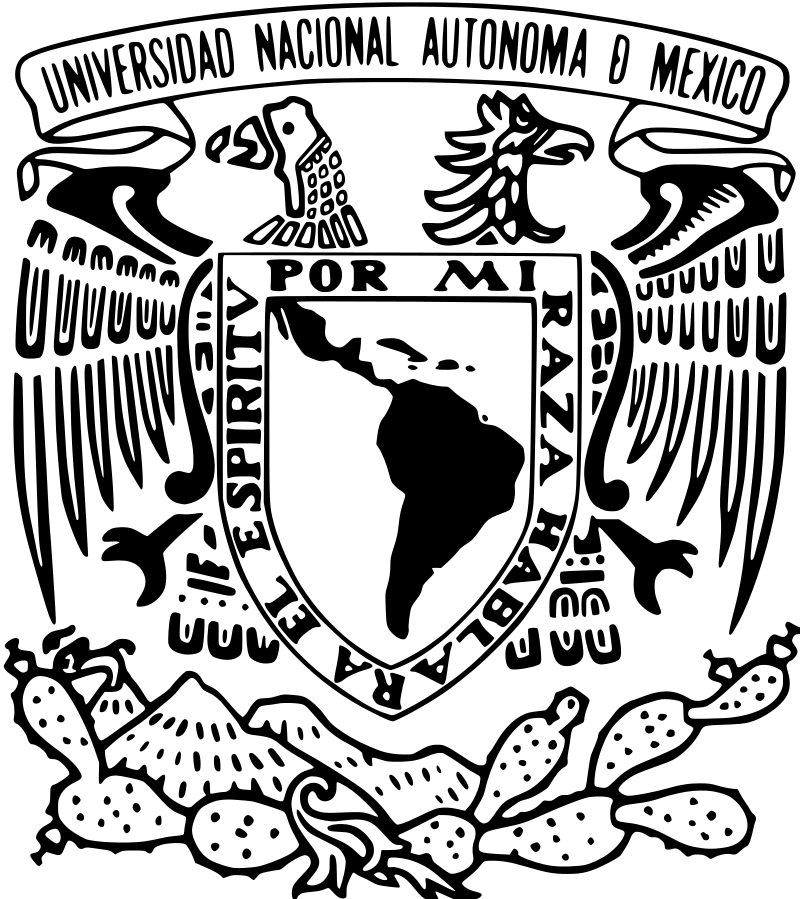
\includegraphics[width=\linewidth]{Escudo_UNAM.png}
\end{minipage}
\begin{minipage}[ht]{0.7\linewidth}
    \centering
    \bf{
    \Huge Universidad Nacional Autónoma de México. \\ 
    \Huge Facultad de Ciencias. \\ 
     Laboratorio de Fenómenos Colectivos.\\
    Práctica : Propiedades térmicas. \\
    %inserten sus nombres xD%
    L. S. Erick A.$^1$\\
    }
\end{minipage}
\begin{minipage}[ht]{0.14\linewidth}
  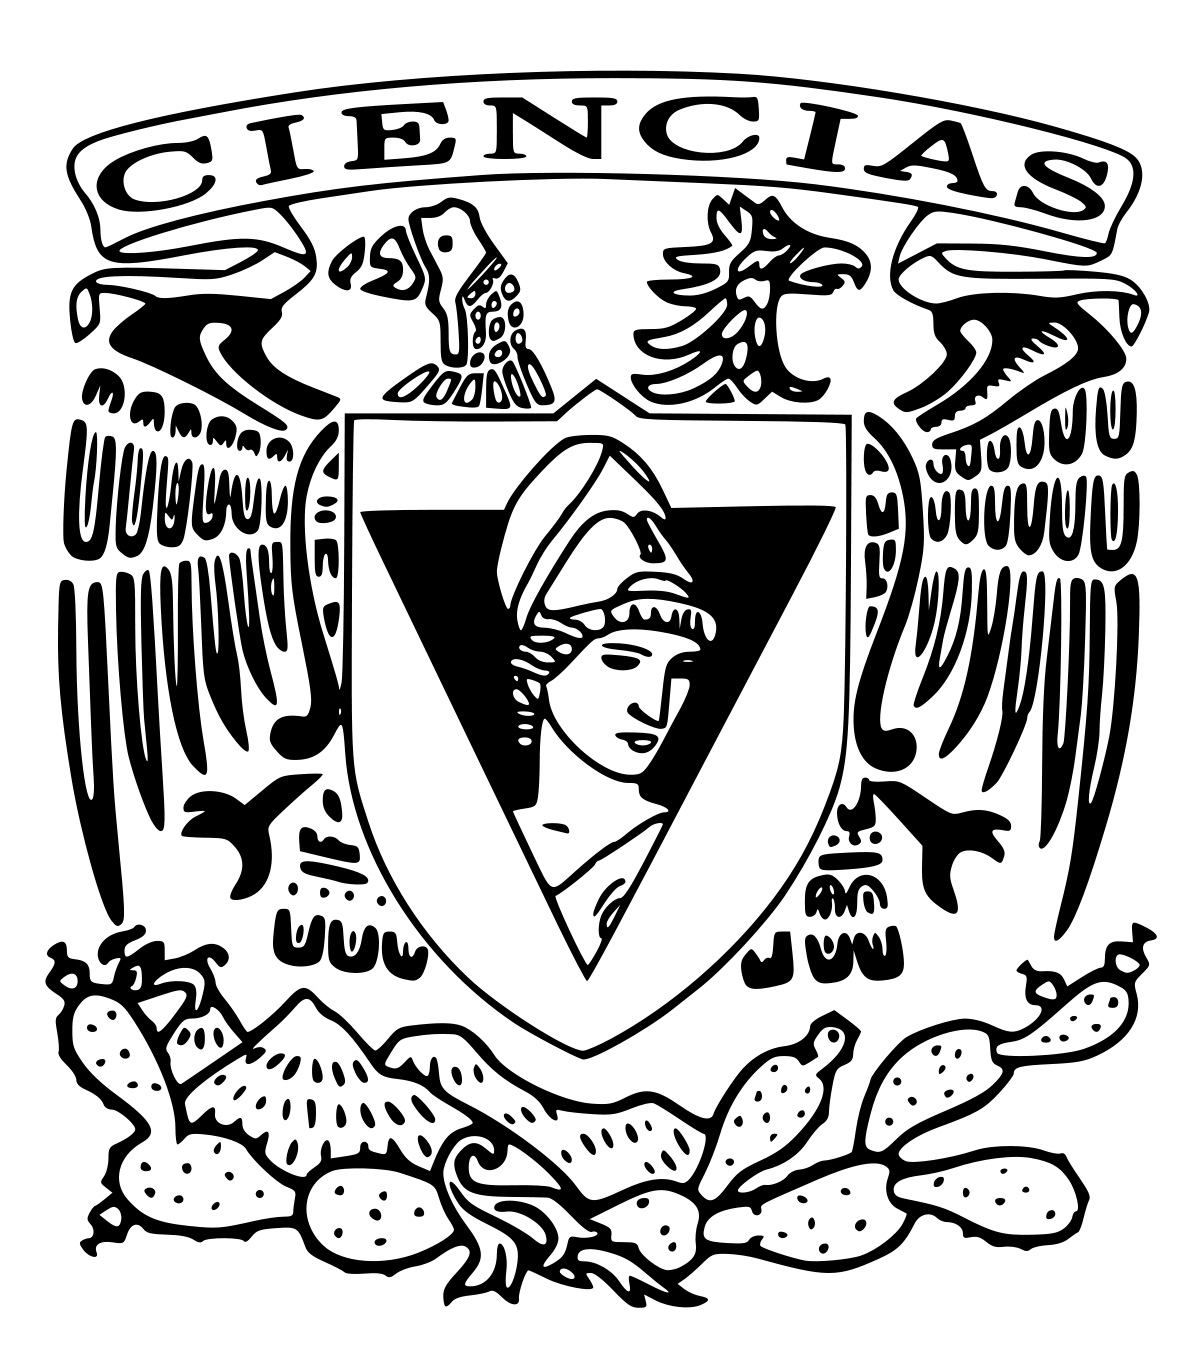
\includegraphics[width=1.01\linewidth]{Escudo_FCiencias.png}
\end{minipage}


\section{Resumen.}
\input{Resumen}

\section{Introducción.}
   \subsection{Objetivos}
        \begin{itemize}
            \item Conocer el calor latente de fusión del hielo.
            \item Conocer El coeficiente de dilatación del aluminio, cobre, acero y agua.
        \end{itemize}

    \subsection{Conceptos Clave}
        \begin{itemize}
            \item Calor Latente de Fusión,
            \item Coeficiente de Dilatación.
        \end{itemize}


    \subsection{Marco teórico.}
        
        El calorímetro es una herramienta utilizada para medir el calor presente en reacciones químicas, procesos de fusión, entre otras. Por su construcción esta herramienta es capaz de aislar termodinámicamente, siendo una pared adiabática, la materia dentro de ésta; este aislamiento permite, con ayuda de un termómetro, medir la variación de la temperatura para poder calcular el calor ganado o perdido de la materia dentro de dicha herramienta. Se conocen calorímetrosa de \textit{poliestireno}, \textit{acero inoxidable}, \textit{de bomba}, y el de \textit{diferencial de barrido}. \cite{Calorímetro}
        
        El calor latente de fusión es una constante, distinta para cada líquido, que se define como la cantidad de energía requerida para transformar un kilogramo de masa sólida a su fase líquida, cuando ésta ya ha alcanzado su temperatura de fusión; de la definición de calor $Q = m \cdot L_{f}$, obtenemos:
        \begin{equation}
            L_{f} = \frac{Q}{m}
        \end{equation}
        
        Donde Q es la energía absorbida por unidad de masa, la variable m es la masa y $L_{f}$ es el "Calor lantente de fusión". \cite{CalorLatente}

        El coeficiente de dilatación es una constante, enciertas condiciones, propia de los materiales, la cual mide cuánto se expande o contrae un material al experimentar un cambio de la temperatura. Cuantifica así el relativo cambio en su longitud, área ó volúmen. Al cambio en su longitud se le llama \textit{dilatación lineal ($\alpha$)}. Matemáticamente se representa como: 
        \begin{equation}
            \alpha = \frac{1}{L_{0}}\frac{\Delta L}{ \Delta T}
        \end{equation}
        El cambio en su área se le define como \textit{dilatación superficial ($\beta$)}, dada por:
        \begin{equation}
            \beta = \frac{1}{A_{0}}\frac{\Delta A}{ \Delta T}
        \end{equation}
        Mientras que al cambio del volumen se nombra \textit{dilatación volumétrica ($\gamma$)}, conocida como:
        \begin{equation}
            \gamma = \frac{1}{V_{0}}\frac{\Delta V}{ \Delta T}
        \end{equation} 

        Decimos que en ciertas ocaciones es constante ya que este comportamiento es casi constante dentro de un determinado rango de temperatura. Esto ya que la estructura molecular de los materiales no responde de manera lineal a grandes cambios de temperatura. Para dichas condiciones se calcula aparte el valor de estos coeficientes. \cite{CoeficientesDilatación}

    \subsection{Materiales.}
        \subsubsection{Calor latente de Fusión}
            \begin{itemize}
                \item Báscula electrónica.
                \item Calorímetro.
                \item Termómetro.
                \item Hielo.
                \item Agua.
            \end{itemize}

        \subsubsection{Coeficiente de Dilatación.}
            \begin{itemize}
                \item Tornillo micrométrico.
                \item Vernier.
                \item Balín de metal.
                \item Lingote de Cobre
                \item Lingote de aluminio
                \item Refrigerador.
                \item Reloj.
            \end{itemize}

 
\section{Desarrollo Experimental.}
    \subsection{Calor Latente de Fusión.}
        Se calibró la báscula con la masa del calorímetro. Luego se vertió agua en el calorímetro, se regristró su masa con ayuda de la báscula electrónica , así como su temperatura. Se vertió el hielo en el calorímetro y se dejó disolver en el agua, posteriormente se registró la temperatura de equilirio entre el hielo y el agua.
    
    \subsection{Coeficiente de Dilatación.}
        Se midió la longitud de los lingotes con un vernier, así como la altura y ancho con un tornillo micrométrico. con el tornillo se midió el diámetro del balín. Se guardó el balín y los lingotes en el refrigerador del  aboratorio durante 20 minutos. Luego se registró de nuevo el largo, ancho y diámetro del balín. 

 

\section{Análisis experimental.}
\subsection{CAlor latente de fusión.}

Veamos qué, 

\section{Conclusión.}
\input{Conclusión}

\section{Bibliografía.}
\nocite{*}
\bibliographystyle{acm}
\bibliography{Bibliografía}

\end{document}
